\appendix

\section{Additional Results}




\subsection{Photo Finishing Tuning Results on FiveK Dataset}
\label{sec:appen_a2}
We show more \taskPFT visualization results on the FiveK-Target evaluation dataset in Fig.~\ref{fig:pft_vis_supp}, showcasing its superior performance in terms of color and brightness compared to all other methods.
\begin{figure*}[ht]
\centering
  \includegraphics[width=\textwidth]{figures/appendix-tuning-results-v1.pdf}
  \caption{Additional results on \taskPFT task.}
  \label{fig:pft_vis_supp}
\end{figure*}

\begin{figure*}[ht]
\centering
  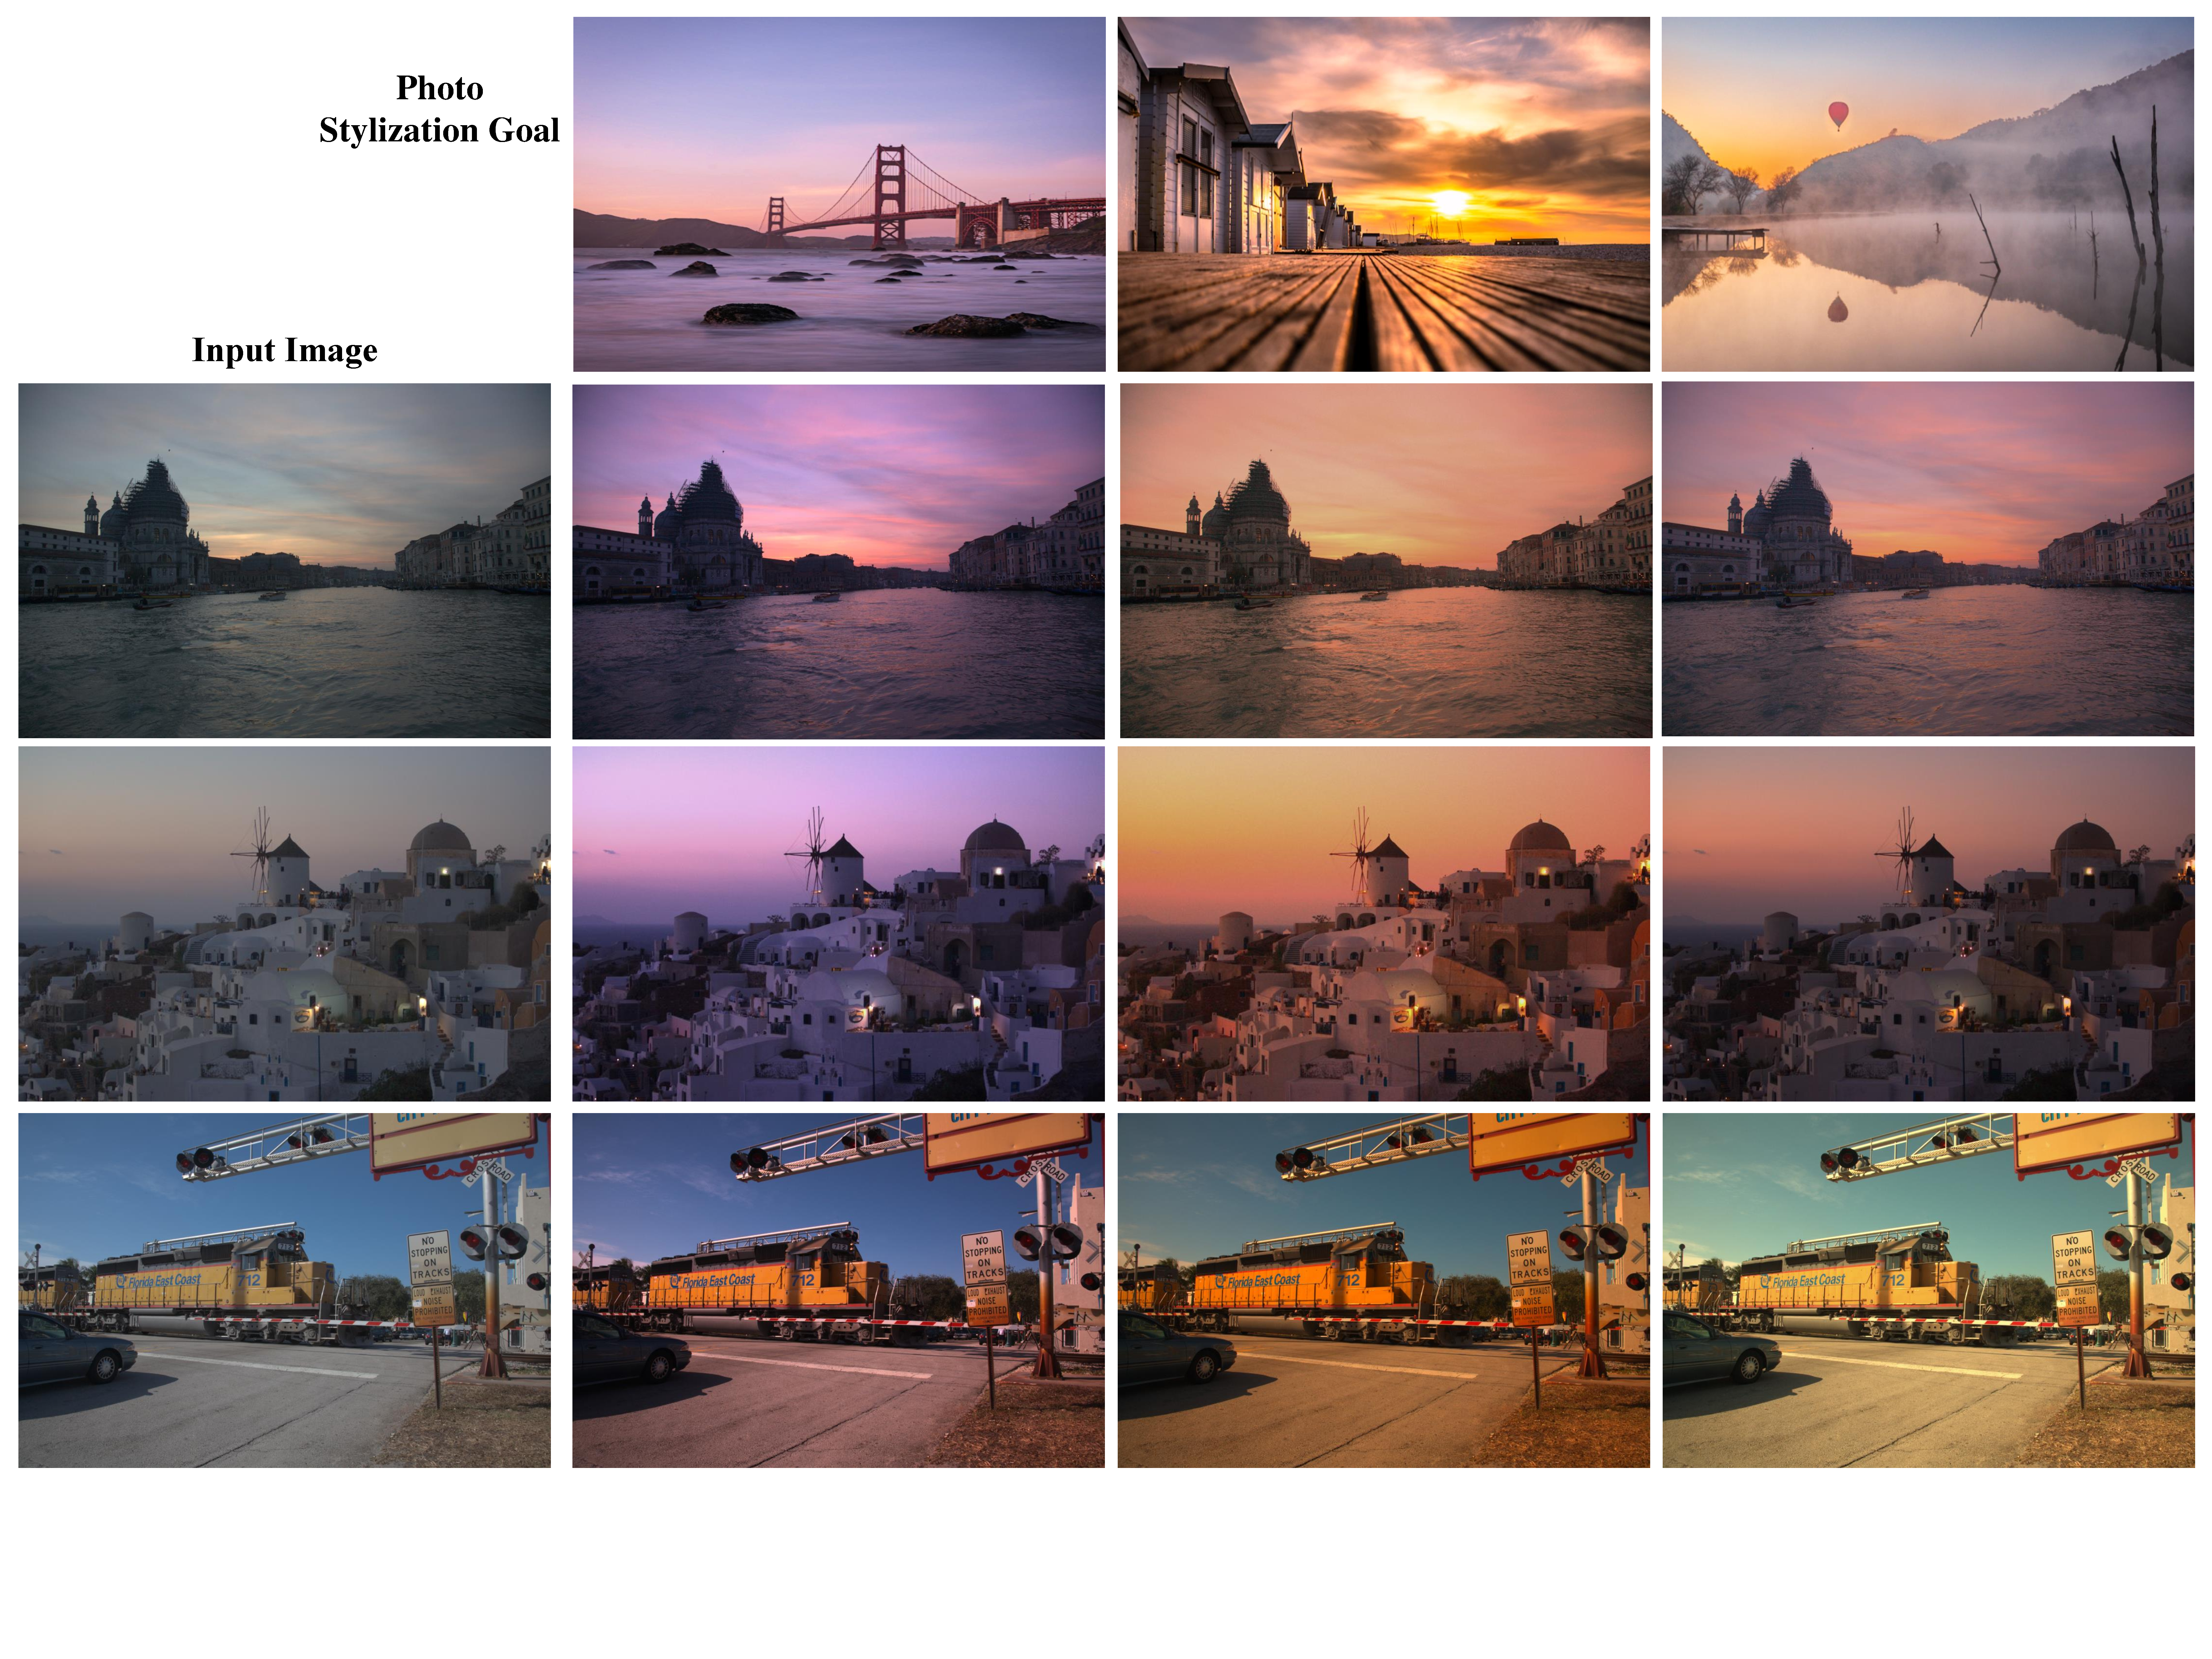
\includegraphics[width=\textwidth]{figures/fig_vis_style_supp.pdf}
  \caption{Additional results on \taskPST task.}
  \label{fig:pst_vis_supp}
\end{figure*}
 
\subsection{Photo Stylization Tuning Results}
\label{sec:appen_a3}
We show more \taskPST visualization results in Fig.~\ref{fig:pst_vis_supp}, showcasing its superior performance in tuning input images to any style goal that is outside the training goal distribution. 


 

\section{Image Processing Pipeline}
The detailed~\pipeline in this paper encompasses various standard operations, including:
\begin{enumerate}[label=(\arabic*)]
    \item Exposure: Adjusts the overall brightness of the image, primarily affecting the amount of light captured. Increasing exposure makes the image brighter while decreasing it makes the image darker. This is useful for correcting overexposed or underexposed photos. This operation includes one slider parameter.
    
    \item Color Balance: Used to adjust the color temperature and tint of an image, altering its overall color feel. Adjusting the color temperature (blue to yellow) and tint (green to magenta) can make the image appear warmer or cooler. This operation includes three slider parameters.
    
    \item Saturation: Controls the intensity of colors in the image. Increasing saturation makes the colors more vivid and lively, whereas decreasing saturation reduces color intensity, making the image appear softer or closer to black and white. This operation includes one slider parameter.

    \item Contrast: Adjusts the difference between the brightest and darkest parts of the image. Increasing contrast makes dark areas darker and bright areas brighter, enhancing the depth and dimension of the image. Decreasing contrast brings these areas closer to mid-grey, reducing the image’s depth. This operation includes one slider parameter.
    
    \item Tone Mapping: This operation compresses a high dynamic range input to a smaller dynamic range, which is affected by the Highlights and Shadows sliders, respectively. Highlights: Adjusts the brightness of the brightest areas of the image without affecting overall exposure. This helps recover details in overexposed areas. Shadows: Adjusts the brightness of the darkest areas, helping reveal details in shadowed regions without changing the overall exposure. This operation includes two slider parameters.
    
     \item Texture: Enhances or reduces the detail and texture in the image without affecting colors. Enhancing texture can make details in the image clearer, while reducing texture can smooth out the image, often used in portrait photos for skin treatment. This operation includes one slider parameter.
    
\end{enumerate}





\section{Additional Implementation Details and Training Strategy}
\label{sec:details}
\subsection{Training Details of TD3 Algorithm}
We state the details of TD3~\cite{fujimoto2018addressing-td3} algorithm training in this subsection. TD3 is an off-policy RL algorithm. When the policy sample transition pair $(s_t,a_t,r_t,s_{t+1},d)$  to form the  replay buffer  $\mathcal{D}$, a gaussian noise is added to encourage exploration: $a= \text{clip}\left(\mu_{\theta}(s) + \epsilon, a_{Low}, a_{High}\right)$, where $ \epsilon \sim \mathcal{N}(0, \sigma) $. We set $\sigma = 0.1$ for a trade-off between exploration and exploitation. 

To compute the target action in Q update target:
\begin{align}\label{eq:qloss1}
L(\phi_{i}) = & ~ \underset{s_t \sim {\mathcal D}}{\mathbb{E}}  \left[ \left( Q_{\phi_i}(s_t,a_t) - \left( r_t + \gamma (1-d) \min_{i=1,2} Q_{\phi_{i, \text{targ}}}(s_{t+1}, a'(s_{t+1}))  \right) \right)^2\right] ,
\end{align}
The next action of $s_{t+1}$ comes from the target policy with a clipped noise, so that incorrect action peak produced by sub-optimal Q value estimation is smoothed out, as in the following equation:
\begin{align}
a'(s_{t+1}) = &~ \text{clip}\left(\mu_{\theta_{\text{targ}}}(s_{t+1}) + \text{clip}(\epsilon_1,-c,c), a_{Low}, a_{High}\right), \;\;\;\;\; \epsilon_1 \sim \mathcal{N}(0, \sigma) 
\end{align}
In this implementation, we set $\epsilon_1 = 0.2$, which is twice the value of $\epsilon$. 
TD3 updates the policy less frequently than the Q-function. We set the policy to update half as frequently as the Q network update. The optimization objectives of the policy are already given in the main paper. To ensure a robust update of the policy and Q network, TD3 adopts an Exponential Moving Average (EMA) strategy to update the target network Q and policy network which is used to compute the Q value target above. 
\begin{align}
\phi_{\text{targ,1}} & \leftarrow \rho \phi_{\text{targ,1}} + (1 - \rho) \phi, \\
\phi_{\text{targ,2}} & \leftarrow \rho \phi_{\text{targ,2}} + (1 - \rho) \phi, \\
\theta_{\text{targ}} & \leftarrow \rho \theta_{\text{targ}} + (1 - \rho) \theta
\end{align}
We set the EMA update rate $\rho = 0.99$ in all our experiments. 
The optimizer is performed using Adam optimizer~\cite{kingma2014adam}  with $(\beta_1, \beta_2) = (0.9, 0.999)$. We set the learning rate to specific values for policy and value network, that is, 1e-4 for action and 2e-4 for Q network. We set batch size as 64 for both \taskPFT and \taskPST experiments. We set the discount factor $\gamma = 0.9$.
All experiments are conducted on NVIDIA RTX 4090 GPUs.
Furthermore, we implement the CMAES method~\cite{tseng2019hyperparameter} based on open-source framework~\cite{pymoo}.



\subsection{Other Training Details}

\noindent\textbf{Reward design.} For our detailed reward design, as described in Sec.~\ref{sec:3.4}, we utilize the PSNR metric of consecutive steps for \taskPFT. In \taskPST, we adopt the style score as the main reward and add a content negative reward to prevent the policy from taking drastic actions that hinder photo stylization quality. Specifically, we set $\lambda_0$ and $\lambda_1$ in $\text{StyleScore}_t$ to 100 and 50, respectively, and set $\lambda_2 = 0.5$. For the VGG features selected to compute the style score, we follow \cite{huang2017arbitrary-adain} to set $N_S = N_C = 4$, selecting $\text{relu\_\{1...4\}\_1}$ features to form $\{F_i\}_{i=1...4}$, which is then used to compute then gram matrix and the content regularization term.

\noindent\textbf{RL termination.} Since our RL policy freely explores the \pipeline parameter space, we need to terminate the current episode if the state collapses, meaning the policy outputs parameters that render an abnormal image. Specifically, we calculate the average pixel intensity of the image $I_t$ as $\mathcal{I}_t$ and set this value to be within the range of $\mathcal{I}_{min}$ and $\mathcal{I}_{max}$. For each rollout, if $\mathcal{I}_t$ is out of range, we terminate the state and do not save it to our replay buffer $\mathcal{D}$.

\noindent\textbf{Network architecture.} Our approach learns an end-to-end policy that maps from input images and goal specifications to the next action to take (the next parameters of the \pipeline.) The state representation is $s_t$ as described in Sec.~\ref{sec:3.3}, which is fed into a 4-layer multi-layer perceptron network (MLP), with a continuous action space of 9 parameters. Each hidden layer of the MLP network is of width 512.




\subsection{Baselines Implementation Details}
\noindent\textbf{Implementation details for CMAES~\cite{hansen2006cma, mosleh2020hardware}.} 
CMAES is a gradient-free search (zeroth order optimization) method using an evolution strategy.  As \cite{mosleh2020hardware} does not provide code, we implemented CMAES using the pymoo library~\cite{pymoo}, enabling parallel execution on multi-core CPUs and achieving reasonable performance. This baseline does not require training.


\noindent\textbf{Implementation details for Cascaded Proxy~\cite{tseng2022neural}.} 
For proxy network training, we followed the architecture in \cite{tseng2022neural}, using 3 consecutive 1 $\times$ 1 convolutions for pointwise ISP operations and 5 consecutive 3 $\times$ 3 convolutions for areawise operations. We trained with the Adam optimizer, a learning rate of 1e-4, a batch size of 512, and 100 epochs, as recommended. Camera metadata was extracted from DNG files, as described in \cite{tseng2022neural}.
Since \cite{tseng2022neural} does not release its dataset, we used the MIT-Adobe FiveK dataset, as in our method. Following Section 5 of \cite{tseng2022neural}, we used 1,000 raw images from FiveK and sampled 100 points for each ISP hyperparameter.


\noindent\textbf{Implementation details for Monolithic Proxy~\cite{tseng2019hyperparameter}.} 
The architecture uses a single UNet to approximate the ISP pipeline, with hyperparameters conditioned by concatenating extra planes to the features. We trained the proxy with the Adam optimizer, a learning rate of 1e-4, a batch size of 512, and 100 epochs.
The training set generation and first-order optimization method are the same as for \cite{tseng2022neural}.






% \section{additional ablation}

\section{Detailed Content of the User Study}
\label{sec:sup-user-study}
We conduct a human subject study on the user preference among results of methods for photo stylization tuning given target style images. In this appendix section, we provide the original questions that we used to ask for users' feedback.

For each of the 20 questions in our user study, the order of the methods was randomized and labeled as A, B, C, and D to ensure the anonymity of the techniques used. Participants were not aware of which method corresponded to each label, eliminating any potential bias in their selections. The prompt for all questions remained consistent: ``Among the four images on the right (labeled A, B, C, and D), which one(s) most closely resembles the target image on the left? You may select up to two images if you believe they are equally similar to the target image. Otherwise, please choose only one.''

Detailed below are the options provided for each of the 20 questions.


\begin{figure}[ht]
    \centering
    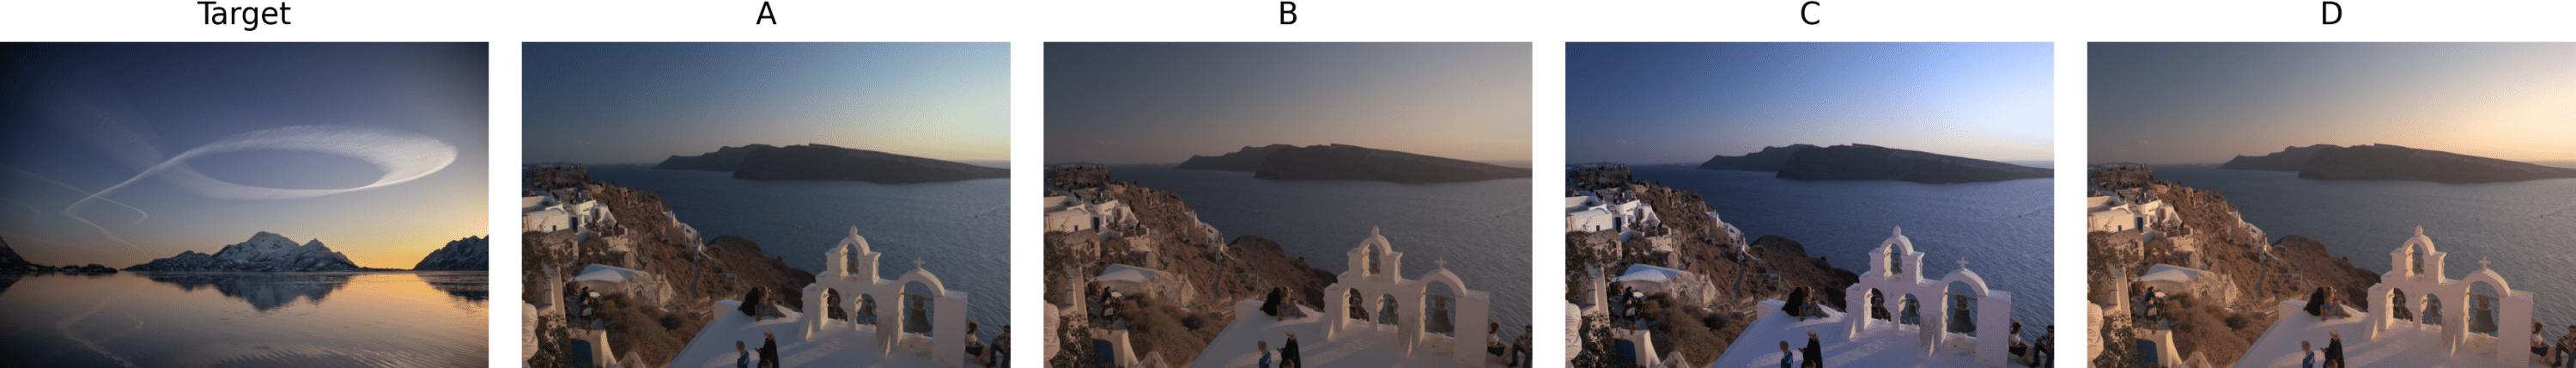
\includegraphics[width=1\linewidth]{figures/user_study/question_1.png}
    \caption{Options in question 1 of our user study.}
    \label{fig:appendix-user-study-q1}
\end{figure}

\begin{figure}[ht]
    \centering
    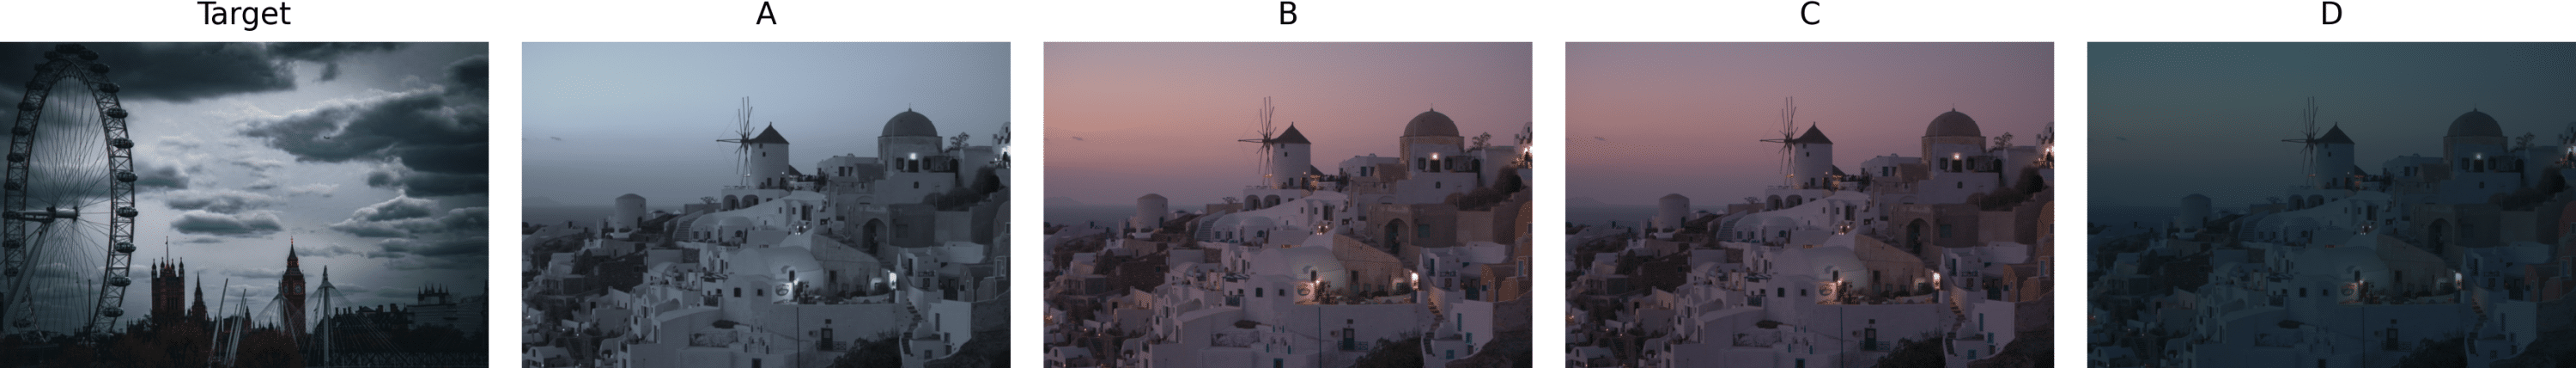
\includegraphics[width=1\linewidth]{figures/user_study/question_2.png}
    \caption{Options in question 2 of our user study.}
    \label{fig:appendix-user-study-q2}
\end{figure}

\begin{figure}[ht]
    \centering
    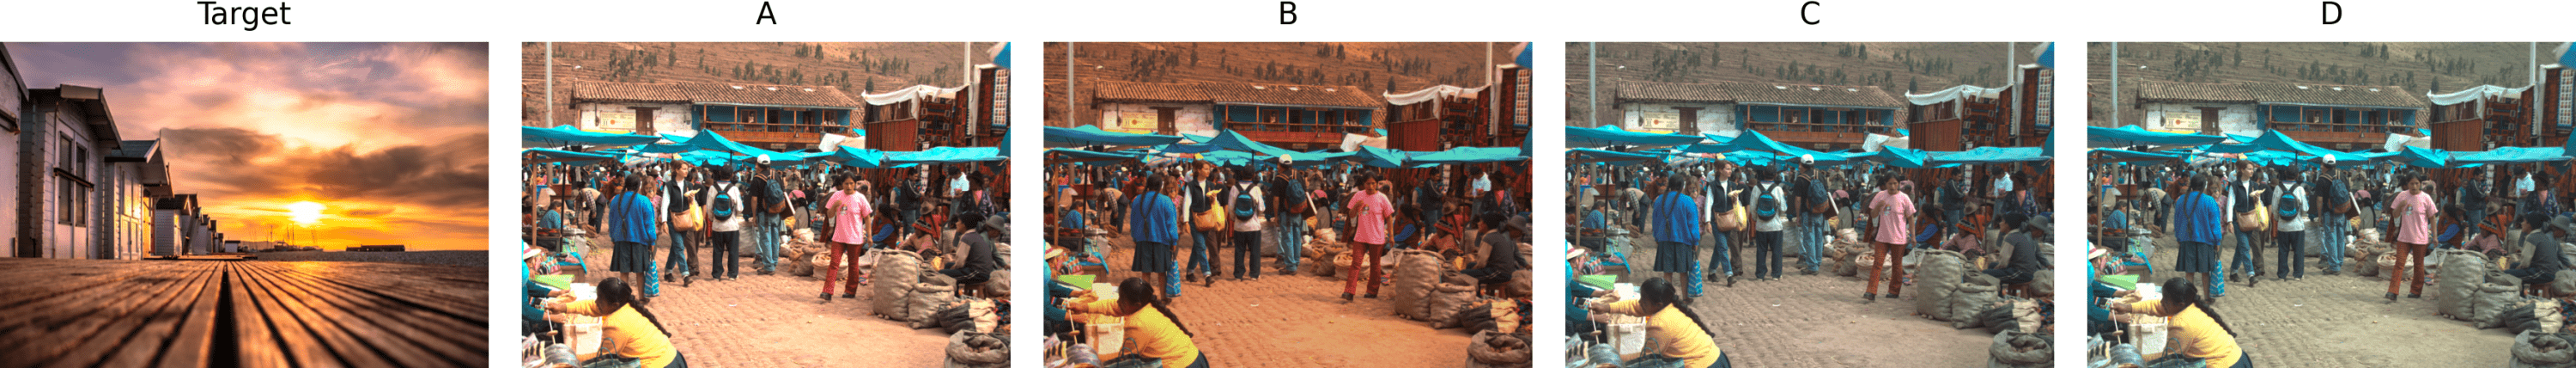
\includegraphics[width=1\linewidth]{figures/user_study/question_3.png}
    \caption{Options in question 3 of our user study.}
    \label{fig:appendix-user-study-q3}
\end{figure}


\begin{figure}[ht]
    \centering
    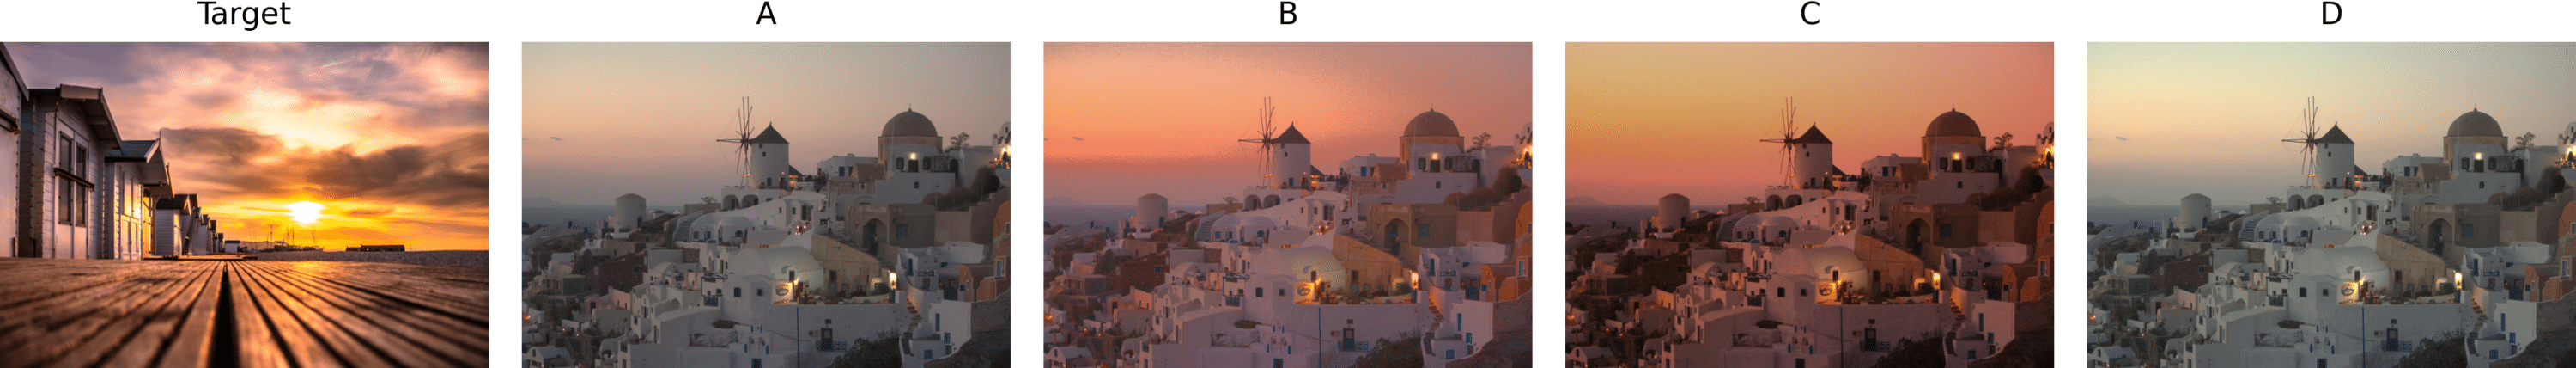
\includegraphics[width=1\linewidth]{figures/user_study/question_4.png}
    \caption{Options in question 4 of our user study.}
    \label{fig:appendix-user-study-q4}
\end{figure}



\begin{figure}[ht]
    \centering
    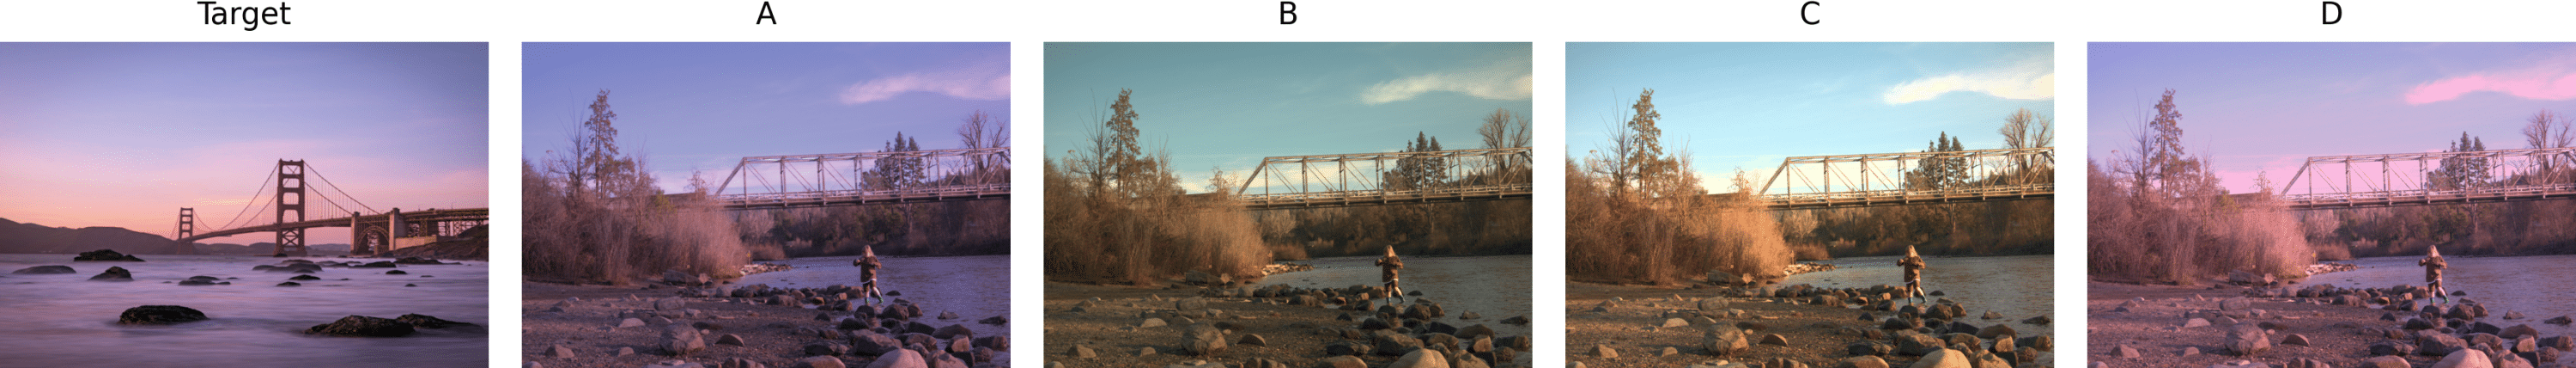
\includegraphics[width=1\linewidth]{figures/user_study/question_5.png}
    \caption{Options in question 5 of our user study.}
    \label{fig:appendix-user-study-q5}
\end{figure}



\begin{figure}[ht]
    \centering
    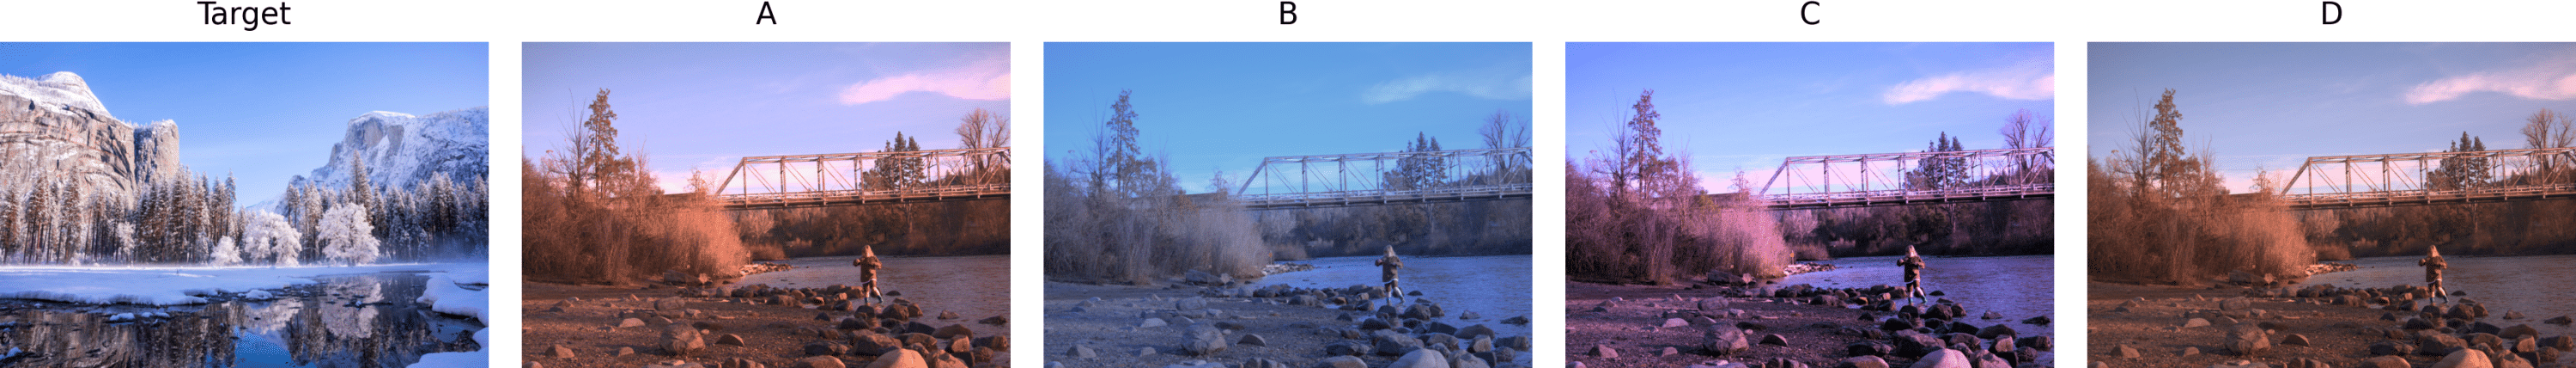
\includegraphics[width=1\linewidth]{figures/user_study/question_6.png}
    \caption{Options in question 6 of our user study.}
    \label{fig:appendix-user-study-q6}
\end{figure}



\begin{figure}[ht]
    \centering
    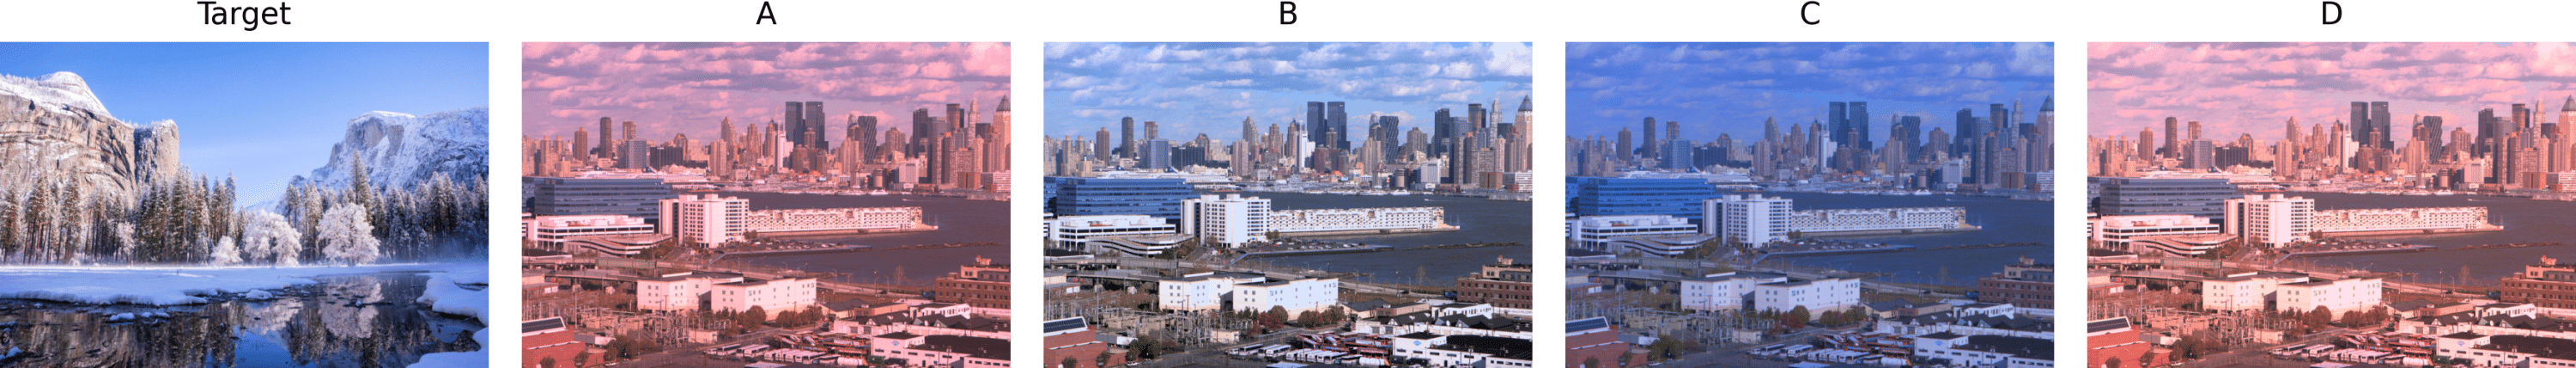
\includegraphics[width=1\linewidth]{figures/user_study/question_7.png}
    \caption{Options in question 7 of our user study.}
    \label{fig:appendix-user-study-q7}
\end{figure}



\begin{figure}[ht]
    \centering
    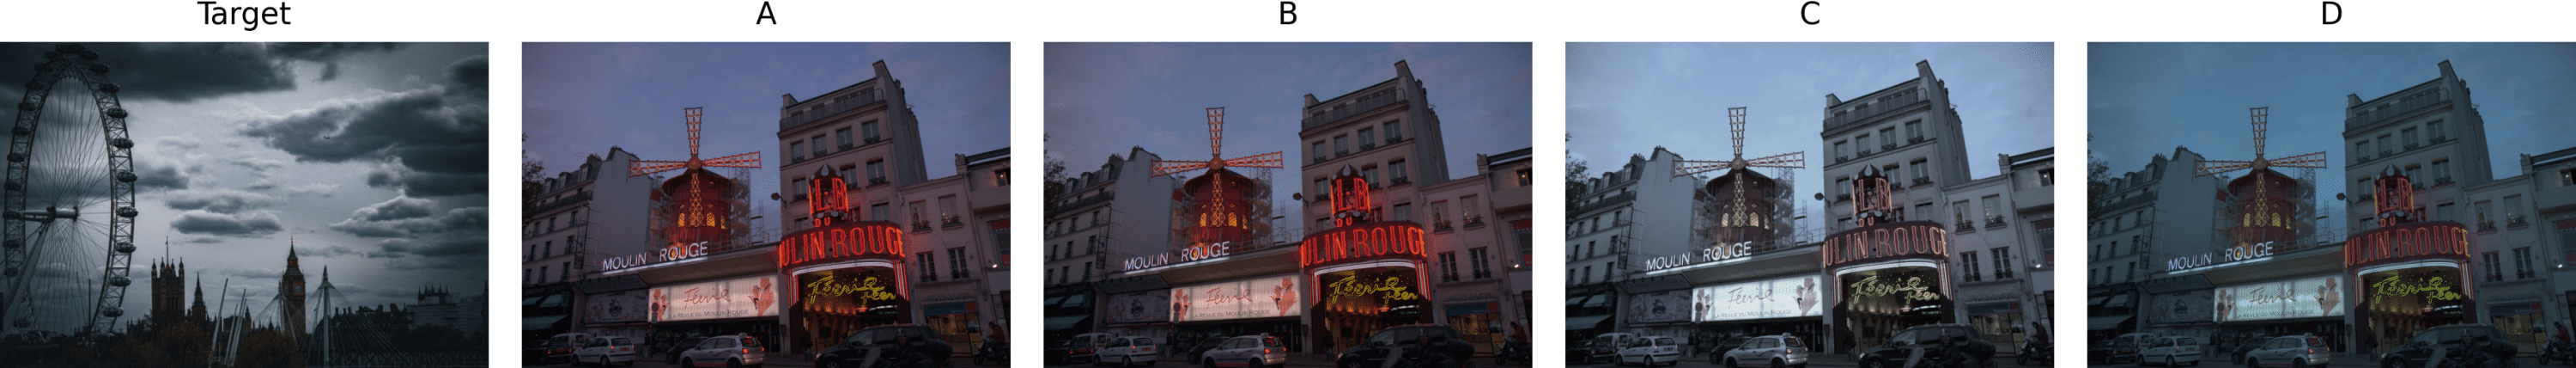
\includegraphics[width=1\linewidth]{figures/user_study/question_8.png}
    \caption{Options in question 8 of our user study.}
    \label{fig:appendix-user-study-q8}
\end{figure}



\begin{figure}[ht]
    \centering
    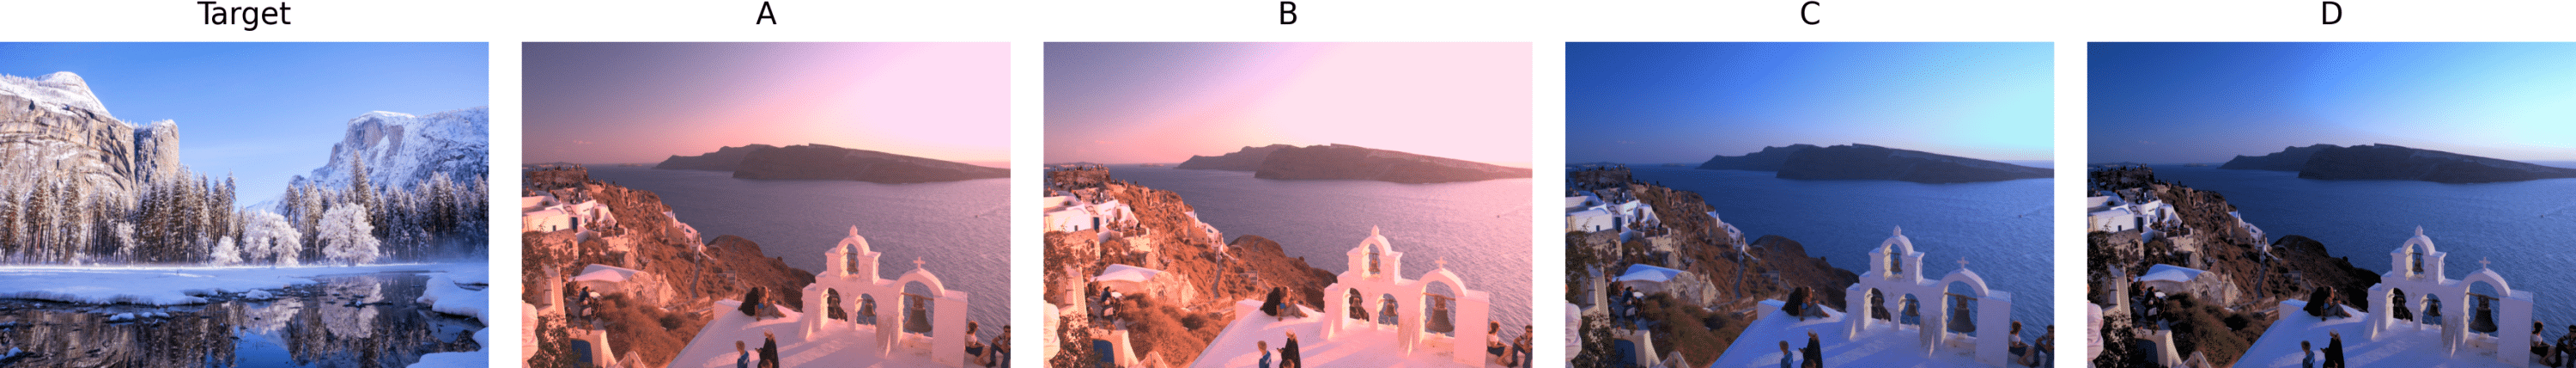
\includegraphics[width=1\linewidth]{figures/user_study/question_9.png}
    \caption{Options in question 9 of our user study.}
    \label{fig:appendix-user-study-q9}
\end{figure}



\begin{figure}[ht]
    \centering
    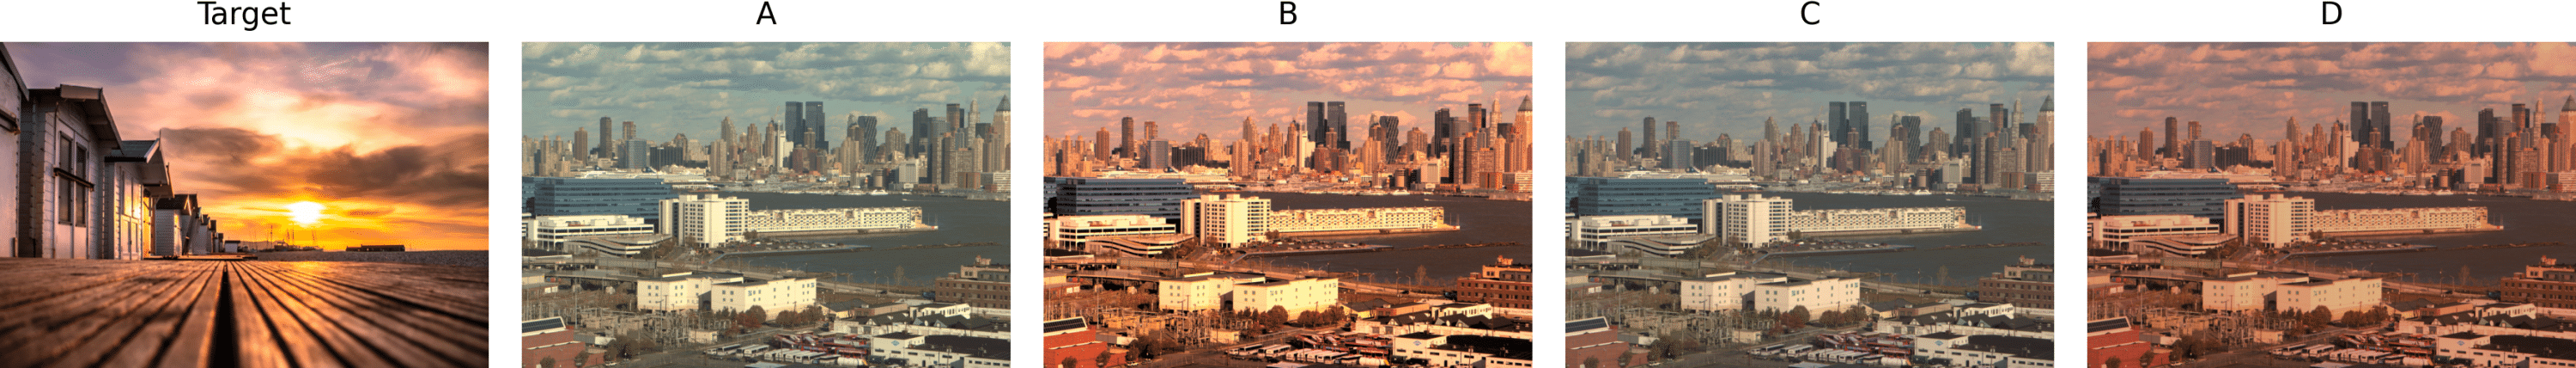
\includegraphics[width=1\linewidth]{figures/user_study/question_10.png}
    \caption{Options in question 10 of our user study.}
    \label{fig:appendix-user-study-q10}
\end{figure}



\begin{figure}[ht]
    \centering
    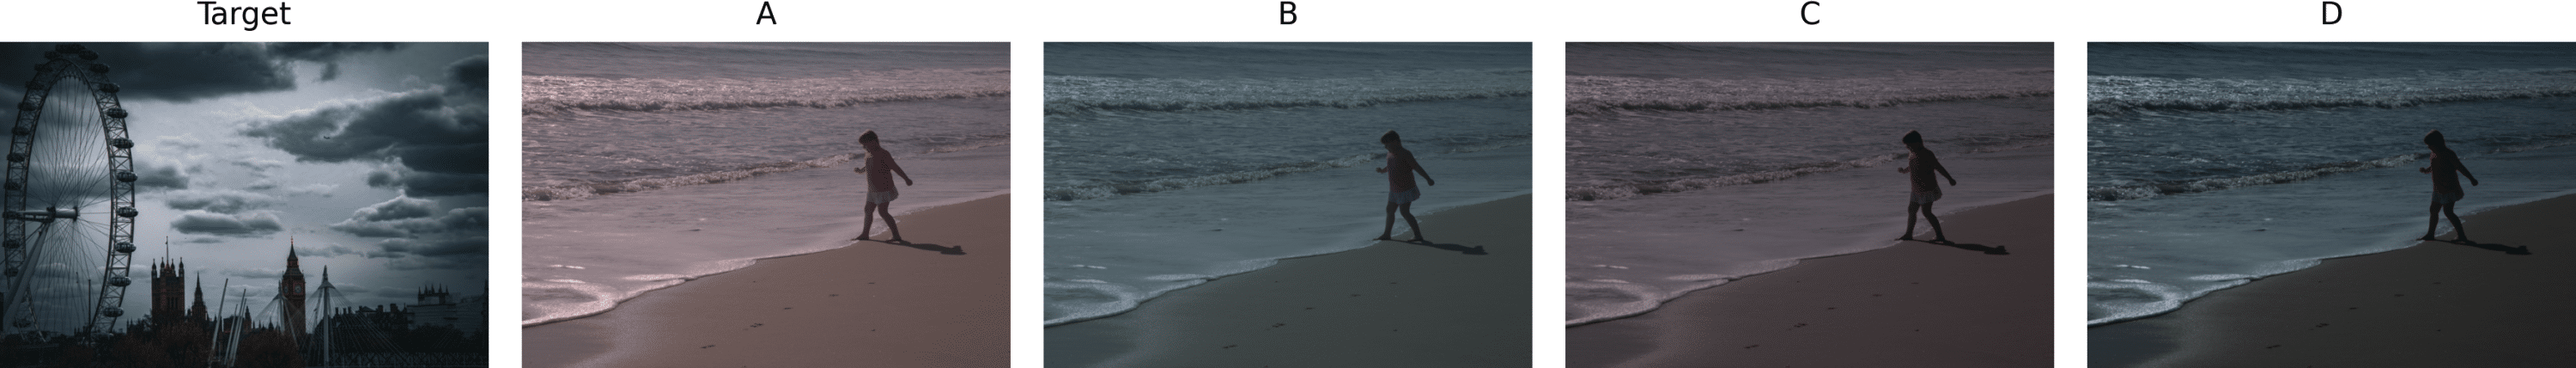
\includegraphics[width=1\linewidth]{figures/user_study/question_11.png}
    \caption{Options in question 11 of our user study.}
    \label{fig:appendix-user-study-q11}
\end{figure}



\begin{figure}[ht]
    \centering
    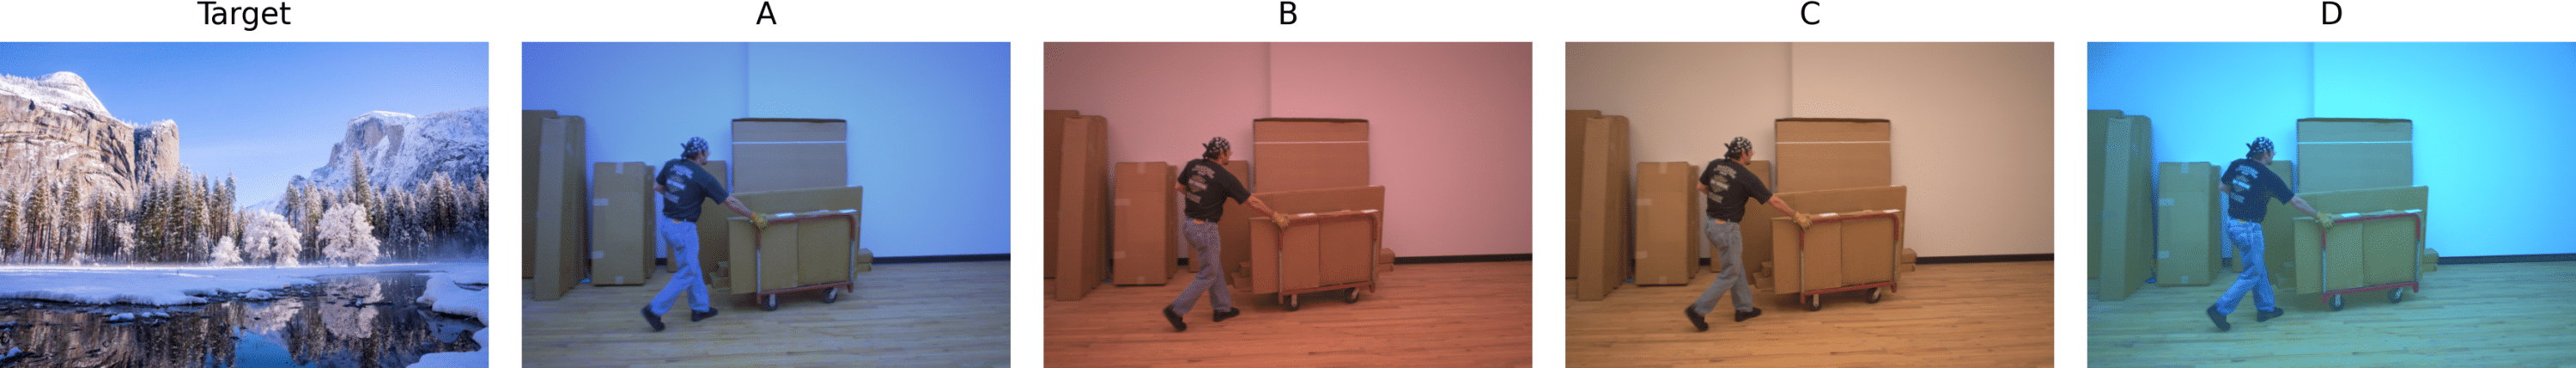
\includegraphics[width=1\linewidth]{figures/user_study/question_12.png}
    \caption{Options in question 12 of our user study.}
    \label{fig:appendix-user-study-q12}
\end{figure}



\begin{figure}[ht]
    \centering
    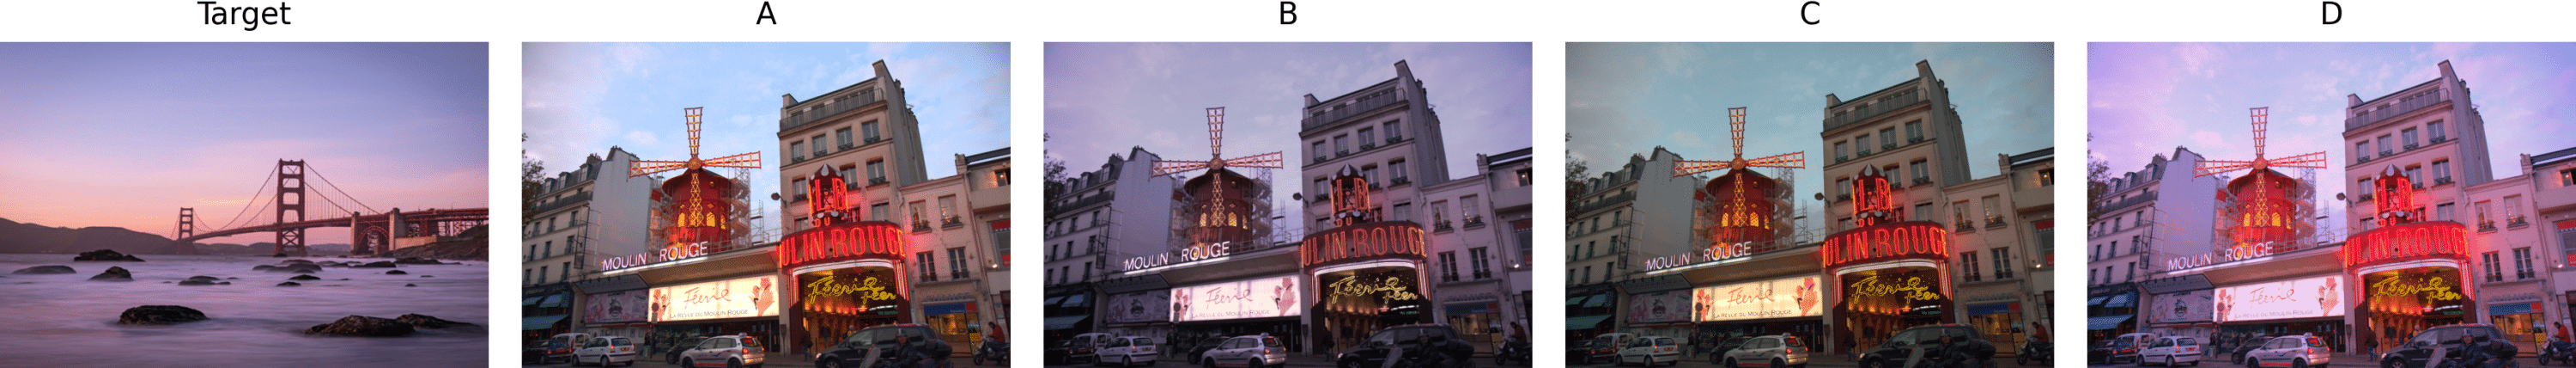
\includegraphics[width=1\linewidth]{figures/user_study/question_13.png}
    \caption{Options in question 13 of our user study.}
    \label{fig:appendix-user-study-q13}
\end{figure}



\begin{figure}[ht]
    \centering
    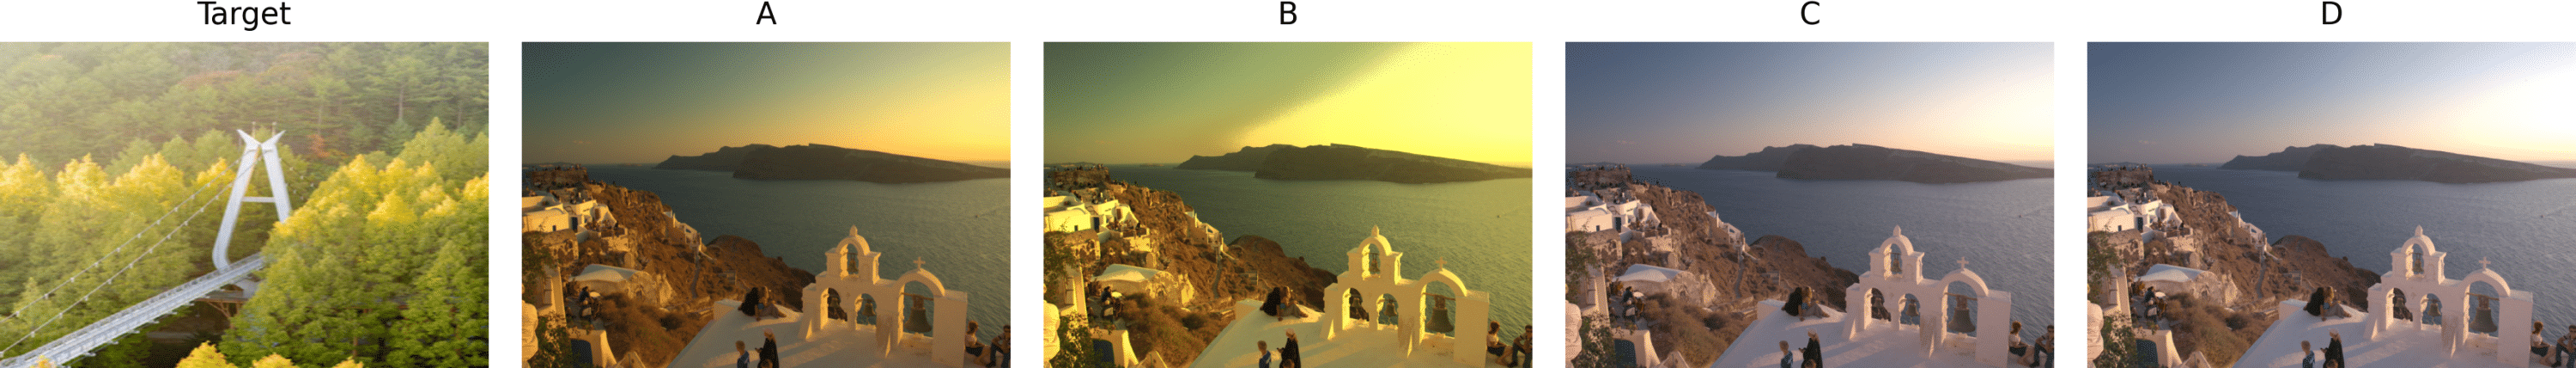
\includegraphics[width=1\linewidth]{figures/user_study/question_14.png}
    \caption{Options in question 14 of our user study.}
    \label{fig:appendix-user-study-q14}
\end{figure}



\begin{figure}[ht]
    \centering
    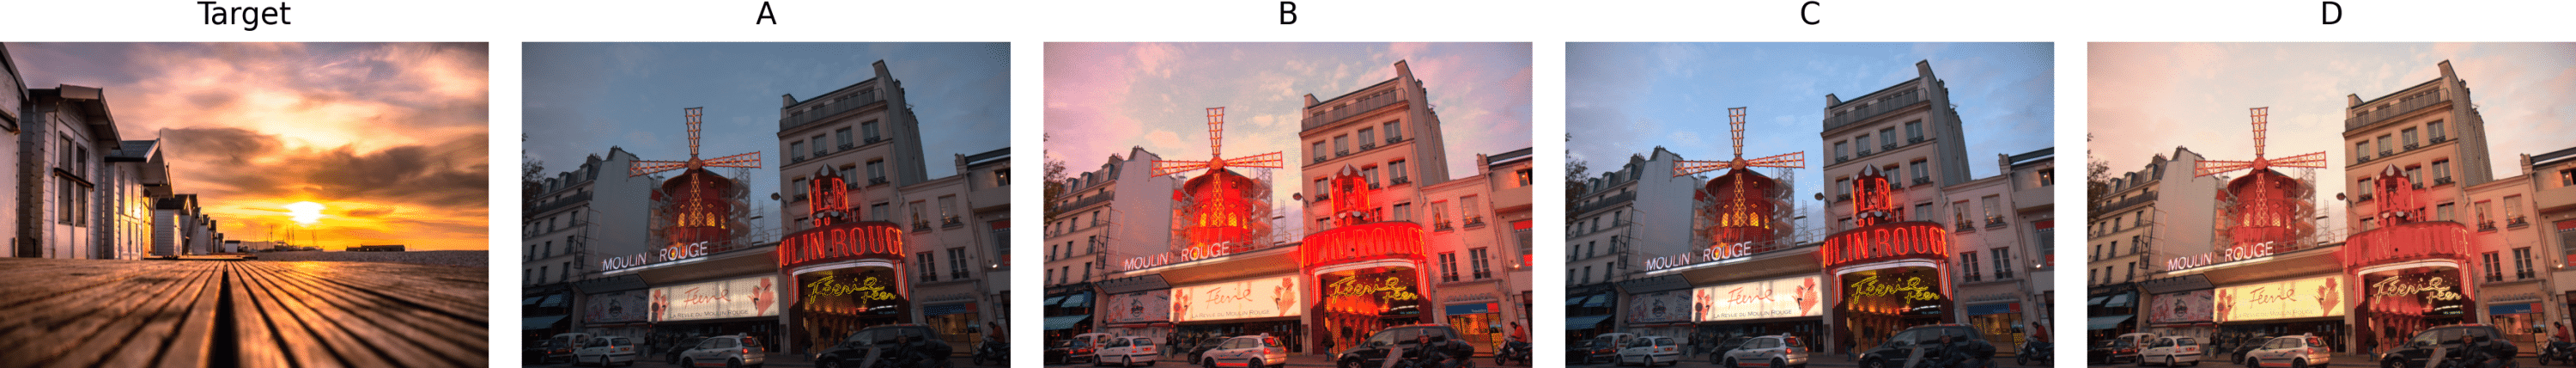
\includegraphics[width=1\linewidth]{figures/user_study/question_15.png}
    \caption{Options in question 15 of our user study.}
    \label{fig:appendix-user-study-q15}
\end{figure}



\begin{figure}[ht]
    \centering
    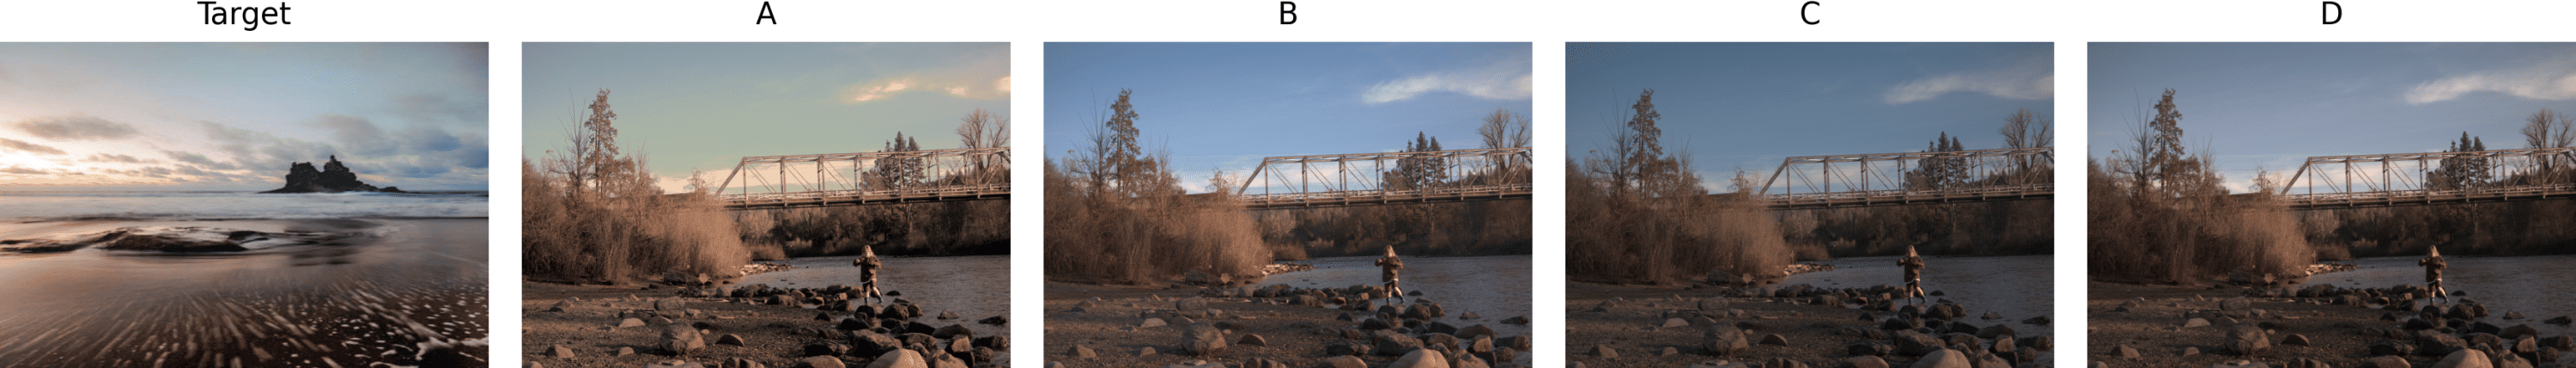
\includegraphics[width=1\linewidth]{figures/user_study/question_16.png}
    \caption{Options in question 16 of our user study.}
    \label{fig:appendix-user-study-q16}
\end{figure}



\begin{figure}[ht]
    \centering
    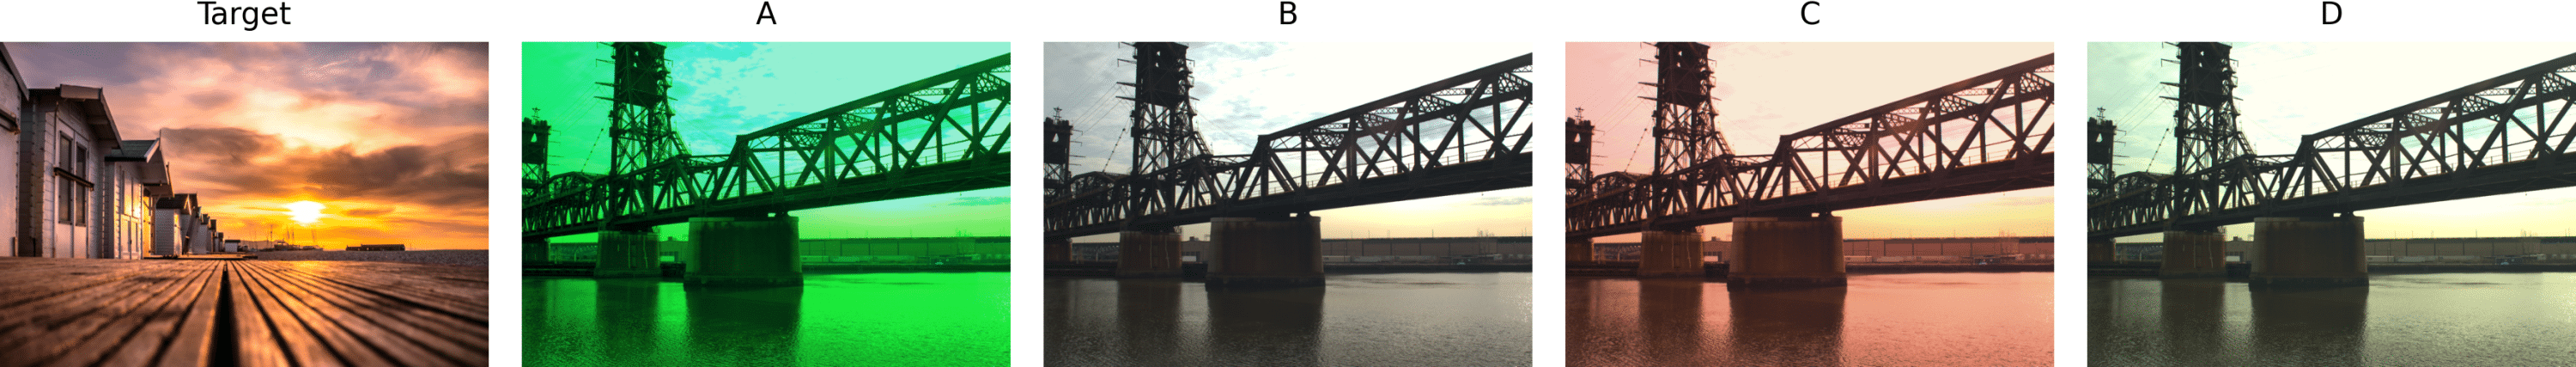
\includegraphics[width=1\linewidth]{figures/user_study/question_17.png}
    \caption{Options in question 17 of our user study.}
    \label{fig:appendix-user-study-q17}
\end{figure}



\begin{figure}[h]
    \centering
    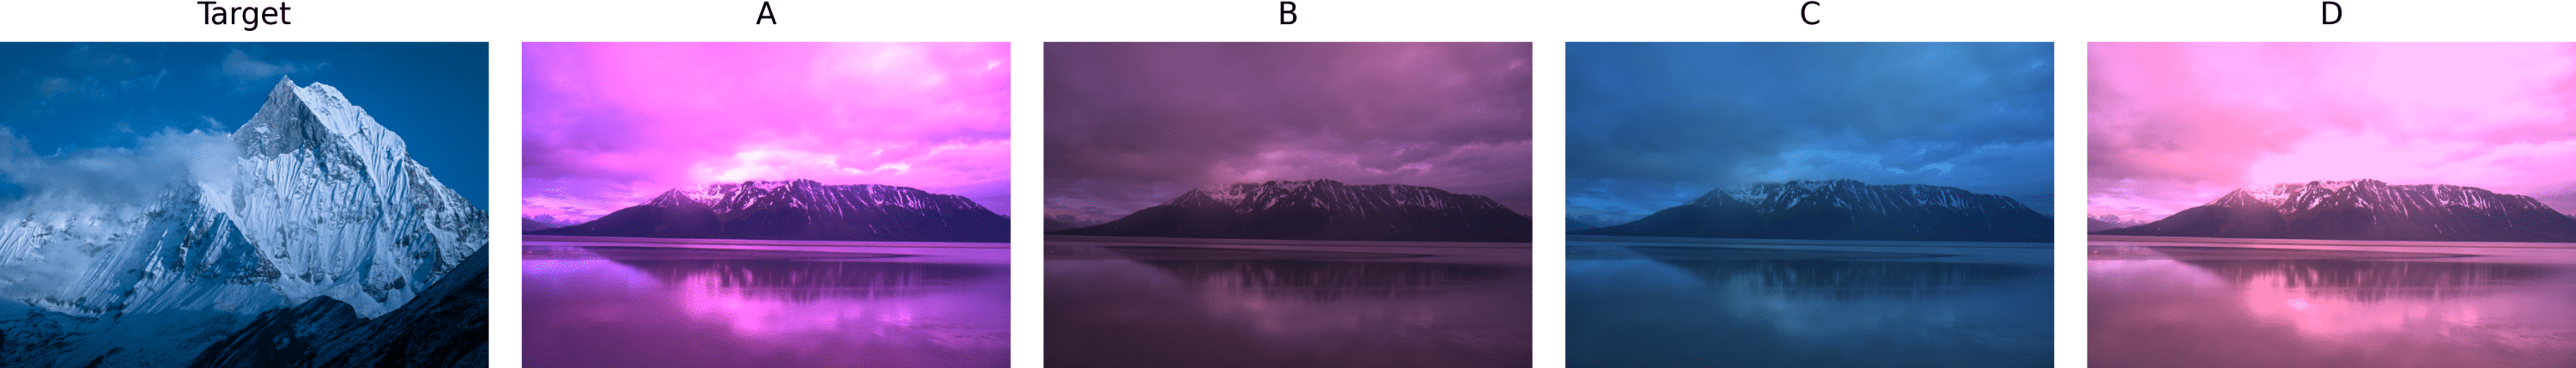
\includegraphics[width=1\linewidth]{figures/user_study/question_18.png}
    \caption{Options in question 18 of our user study.}
    \label{fig:appendix-user-study-q18}
\end{figure}



\begin{figure}[ht]
    \centering
    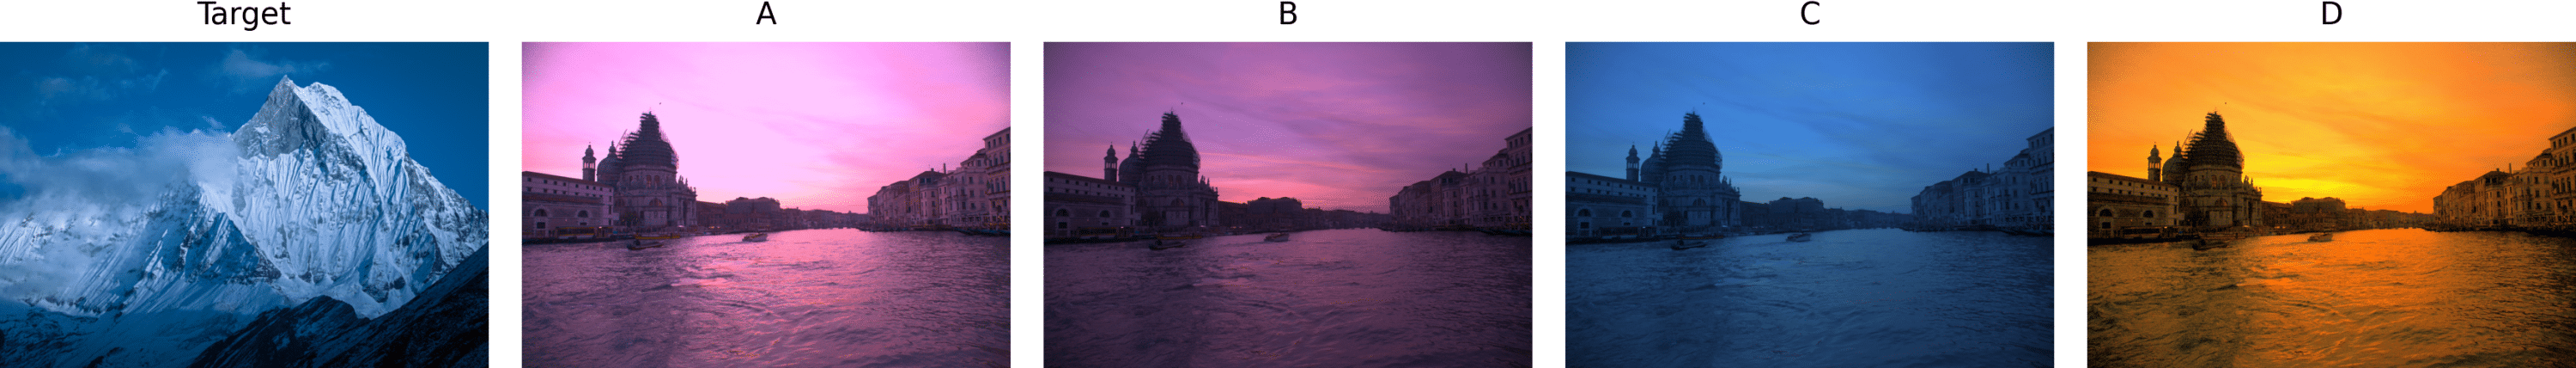
\includegraphics[width=1\linewidth]{figures/user_study/question_19.png}
    \caption{Options in question 19 of our user study.}
    \label{fig:appendix-user-study-q19}
\end{figure}



\begin{figure}[ht]
    \centering
    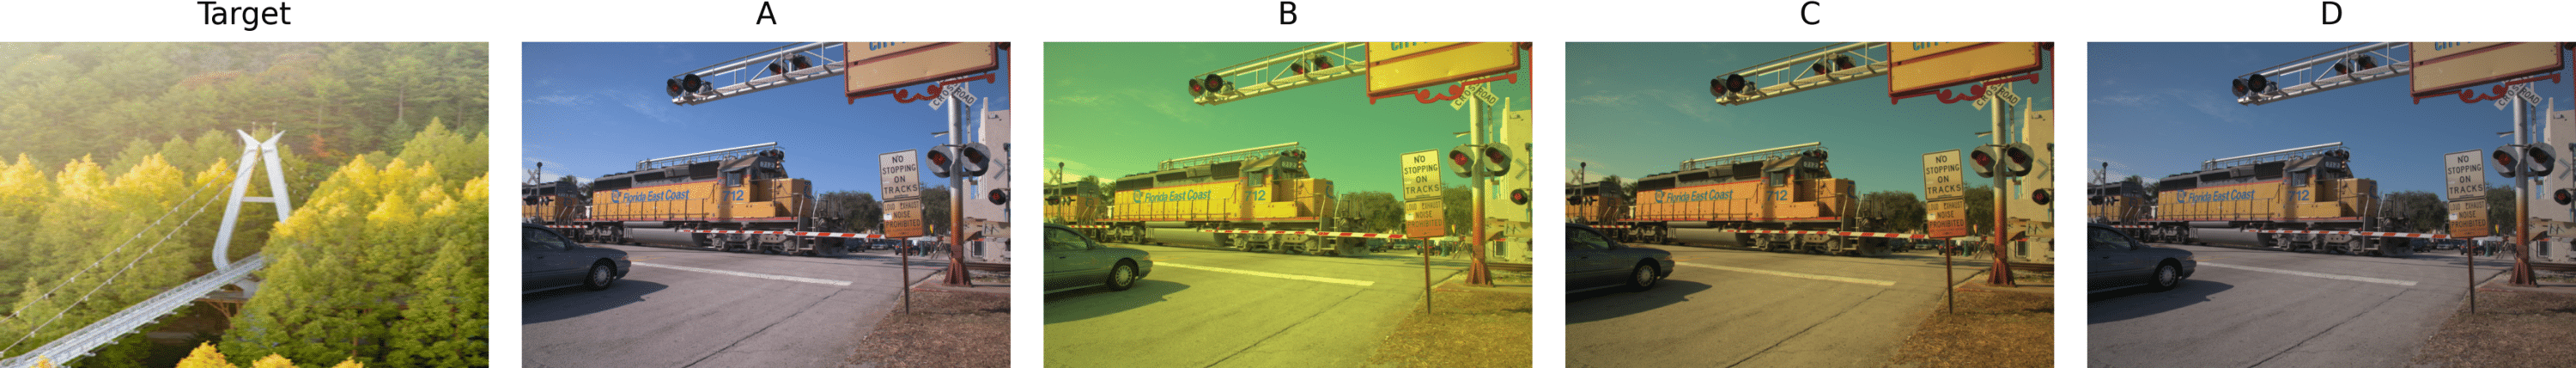
\includegraphics[width=1\linewidth]{figures/user_study/question_20.png}
    \caption{Options in question 20 of our user study.}
    \label{fig:appendix-user-study-q20}
\end{figure}


